\documentclass[preprint,12pt]{elsarticle}
\usepackage{amssymb}
\usepackage{amsmath}
\usepackage{float}
\usepackage{listings}

\newcommand{\inner}[2]{\langle #1 | #2 \rangle}
\newcommand{\R}{\mathbb{R}}
\newcommand{\wij}{W_{ij}}
\newcommand{\loss}{\mathcal{L}}

\journal{Nuclear Instruments and Methods
in Physics Research Section A: Accelerators, Spectrometers,
Detectors and Associated Equipment}

\begin{document}

\begin{frontmatter}

%% \title{Title\tnoteref{label1}}
%% \tnotetext[label1]{}
%% \author{Name\corref{cor1}\fnref{label2}}
%% \ead{email address}
%% \ead[url]{home page}
%% \fntext[label2]{}
%% \cortext[cor1]{}
%% \address{Address\fnref{label3}}
%% \fntext[label3]{}

\title{Latent Variable Clustering for Classification of Events in the AT-TPC}

%% use optional labels to link authors explicitly to addresses:
%% \author[label1,label2]{}
%% \address[label1]{}
%% \address[label2]{}

\author{R.~Solli}
\address{Department of Physics, University of Oslo, POB 1048 Oslo, N-0316 Oslo, Norway}

\author{D.~Bazin}
\address{Department of Physics and Astronomy and Facility for Rare Ion Beams and National Superconducting Cyclotron Facility, Michigan State University, East Lansing, MI 48824, USA}
\author{M.P.~Kuchera}
\address{Physics Department, Davidson College, Davidson, North Carolina, USA}
\author{M.~Hjorth-Jensen}
\address{Department of Physics and Astronomy and Facility for Rare Ion Beams and National Superconducting Cyclotron Facility, Michigan State University, East Lansing, MI 48824, USA}
\address{Department of Physics and Center for Computing in Science Education, University of Oslo, POB 1048 Oslo, N-0316 Oslo, Norway}
\ead{hjensen@frib.msu.edu}
\ead[url]{http://mhjgit.github.io/info/doc/web/}


\begin{abstract}
In this work we introduce the application of convolutional autoencoder neural networks to the analysis of two-dimensional projections of particle tracks from a resonant proton scattering experiment on ${}^{46}$Ar. 
The data we analyze were recorded by an active target time-projection chamber (AT-TPC). Machine learning presents an interesting avenue for researchers operating an AT-TPC, as traditional analysis methods of AT-TPC data are both computationally expensive and fit all particle tracks against the event type of interest. The latter presents a considerable challenge when the space of reactions is not known prior to the analysis. 

We explore the performance of the autoencoder neural networks and a pre-trained VGG16 \cite{Simonyan2014} convolutional neural network on two tasks: a semi-supervised classification task and the unsupervised clustering of particle tracks. On the semi-supervised task, we find that a logistic regression classifier trained on small labelled subsets of the latent space of these models perform very well. On simulated data these classifiers achieve an $f1$ score \cite{Chinchor1992} of $f1>0.95$. The VGG16 latent classifier achieves this result with as few as $N=100$ samples, as does the convolutional autoencoder when trained on the VGG16 representations of the particle tracks. On real data, pre-processed with noise filtering, the same models achieve an $f1>0.7$. For unfiltered real data the models achieve an $f1$ value larger than $0.6$. Both of the previous results were found with the classifiers trained on $N=100$ samples. Furthermore, we found that the autoencoder model reduces the variability in the identification of proton events by $64\%$ from the benchmark logistic regression classifier trained on the VGG16 latent space on real experimental data. 

On the clustering task, we found that a $K$-means algorithm applied to the simulated data in the VGG16 latent space forms almost perfect clusters, with an adjusted rand index \cite{Hubert1985} ($ARI$) $ > 0.8$.  Additionally, the VGG16+K-means approach finds high purity clusters of proton events for real experimental data. We also explore the application of neural networks to clustering by implementing a mixture of autoencoders algorithm. With this model we improved clustering performance on the real experimental data from an $ARI = 0.17$ to an $ARI = 0.40$. However, the neural network clustering suffers from stability issues necessitating further investigations into this approach. 

\end{abstract}

%%Graphical abstract
\begin{graphicalabstract}
%\includegraphics{grabs}
\end{graphicalabstract}

%%Research highlights
\begin{highlights}
\item Research highlight 1
\item Research highlight 2
\end{highlights}

\begin{keyword}
%% keywords here, in the form: keyword \sep keyword

%% PACS codes here, in the form: \PACS code \sep code

%% MSC codes here, in the form: \MSC code \sep code
%% or \MSC[2008] code \sep code (2000 is the default)

\end{keyword}

\end{frontmatter}

\section{Introduction}\label{sec:intro}

\section{Methods}\label{sec:methods}
\subsection{Why machine learning}

\begin{itemize}
    \item Traditional MC methods fall short in two principal ways:
    \begin{itemize}
        \item The computational cost per event is too large given the size of the data-sets
        \item The broken tracks, noisy environment creates bad fit statistics for otherwise useful events. End result is $f1 \sim 0.7 $
    \end{itemize}
\end{itemize}

\subsection{Machine Learning}

\begin{itemize}
    \item Reiterate the aim of unsupervised  clustering of events.
    \item Challenges from a machine learning perspective. 
    \begin{itemize}
        \item Supervised vs. Unsupervised learning
        \item Traditional unupervised - distances in high dimensional spaces etc. 
    \end{itemize}
    \item Digression here to explain some ML concepts? Link back to Conv part of Michelles paper? 
    \item Opportunities presented by: 
    \begin{itemize}
        \item Transfer learning (train on VGG use on AT-TPC)
        \item Compression is understanding (leverage autoencoders) 
    \end{itemize}
    \item Building on Kuchera et. al we investigate the VGG16 networks application. 
    \item Novel contribution by applying clustering autoencoder networks. 
\end{itemize}
\section{Results and Discussions}\label{sec:results}
The principal challenge in the AT-TPC experiments that we are trying to solve is the reliance on labelled samples in the analysis as future experiments may not have as visually dissimilar reaction products  as we observe in the ${}^{46}$Ar experiment.  The  ${}^{46}$Ar experiment does, however, provide a useful example where we can then explore unsupervised techniques. In this chapter, we explore the application of clustering techniques to events represented in latent spaces. 

We begin by exploring a naive K-means approach on the latent space of a pre-trained network. Subsequently, we investigate other clustering methods and two autoencoder based clustering algorithms, as outlined in section \ref{sec:deep_clustering}.

This chapter builds on the previous results from semi-supervised classification. We observe that we can construct high-quality latent spaces. These high-quality spaces facilitate an investigation of clustering techniques. 

The approach for clustering of events is different from the semi-supervised approach in two meaningful ways. First, it is a harder task, as we will demonstrate. The clustering task thus necessitates a more exploratory approach to the problem. Second, as a consequence of the challenge, the focus will be a bit different than for the semi-supervised approach. We will still utilize the same architectures and models starting with a search over the parameter space over which we measure the performance using the adjusted rand score (ARS) and accuracy defined in section \ref{sec:unsupervised_perf} and \ref{sec:supervised_perf}, respectively.

As with chapter  \ref{chap:classification} where we explored the semi-supervised results, we begin this chapter by considering the VGG16 pre-trained model as a benchmark.

Lastly, we note that the focus of this work is mainly on discovering possible avenues for further research. This focus requires a broad scan of possible avenues rather than a rigorous analysis of one specific model.
\subsection{Transfer learning}
As in chapter \ref{ch:architectures}, we also use the VGG16 pre-trained network as a baseline for the clustering performance. We begin by considering a classical K-means approach to clustering. However, the output from the VGG16 network is very high dimensional with output vectors in $\R^{8192}$. One of the primary concerns is then the curse of dimensionality, where the ratio of distances goes to one with increasing dimensionality as shown by \citet{Aggarwal}. However, one of the central caveats to the authors  finding is that the elements are uniformly distributed in the latent space. It is then possible that all the class information lies in some sub-space of the latent data. To investigate this, we perform clustering analysis using the full representation and the $10^2$ first principal components only. 

\subsection{K-means}

We begin by investigating the K-means clustering algorithm on the VGG16 latent space. As in chapter \ref{chap:classification} the VGG16 model is pre-trained on the imagenet dataset creating a set of vectors $\boldsymbol{x} \in \R^{8192}$. To cluster we use \lstinline{scikit-learn} implementation of the K-means algorithm, with default parameters \cite{Pedregosa2011}. The results of the clustering runs are included in table \ref{tab:clstr_vgg}. We observe that we are able to attain near-perfect clustering on simulated data and that there is a sharp decline in performance as we add noise by moving to the filtered and full datasets. 

\begin{table}[H]
\centering 
\caption[K-means on pre-trained model]{K-means clustering results on AT-TPC event data. We observe that the performance predictably decreases with the amount of noise in the data.}\label{tab:clstr_vgg}
\begin{tabular}{lll}
\toprule
{} & Accuracy &   ARI \\
\midrule
Simulated &     0.97 &  0.89 \\
Filtered  &     0.74 &  0.39 \\
Raw       &     0.59 &  0.17 \\
\bottomrule
\end{tabular}

\end{table}

In addition to the performance measures reported in table \ref{tab:clstr_vgg}, it is interesting to observe which samples are being wrongly assigned. We achieve this by tabulating the assignments of samples relative to their ground truth labels. From these tables, we can infer which classes are more or less entangled with others. We tabulate the results for each dataset is in figure \ref{fig:clster_confmat}. We observe that the proton class is consistently assigned in a pure cluster. Purity is inferred by how much spread there is in the column between the ground truth labels. A high-quality cluster will, in addition to being pure, also capture most entries the class represented by the cluster. For example, consider the row corresponding to the proton class in figure \ref{fig:clster_confmat}. The column corresponding to the largest entry in the proton row has zero other predicted classes in it. From this, we conclude that the proton cluster is a high quality, high purity cluster. 

\begin{figure}
\centering

	\subfloat{
	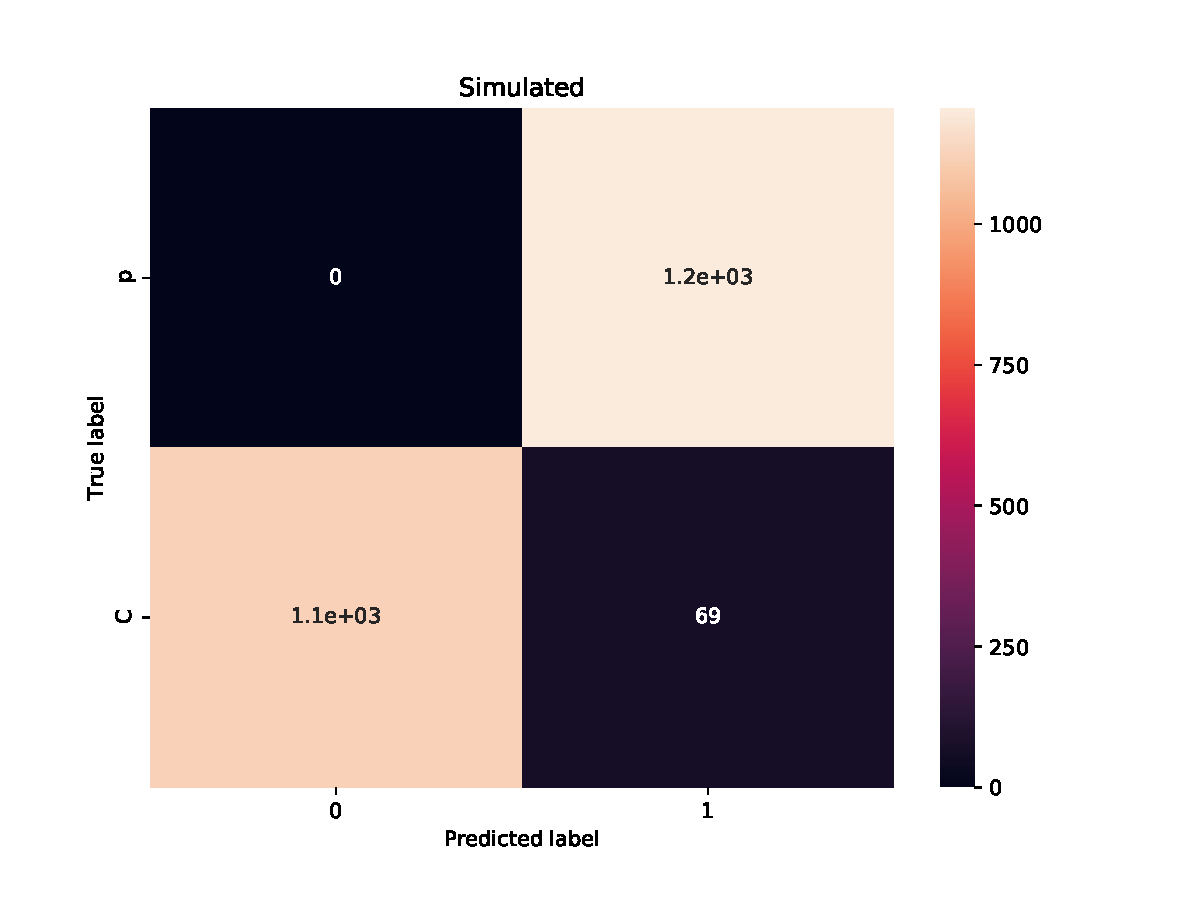
\includegraphics[width=0.35\textwidth]{./plots/Simulatedvgg_pca_conf_mat.pdf}

}
	\hspace{-1cm}
	\subfloat{
	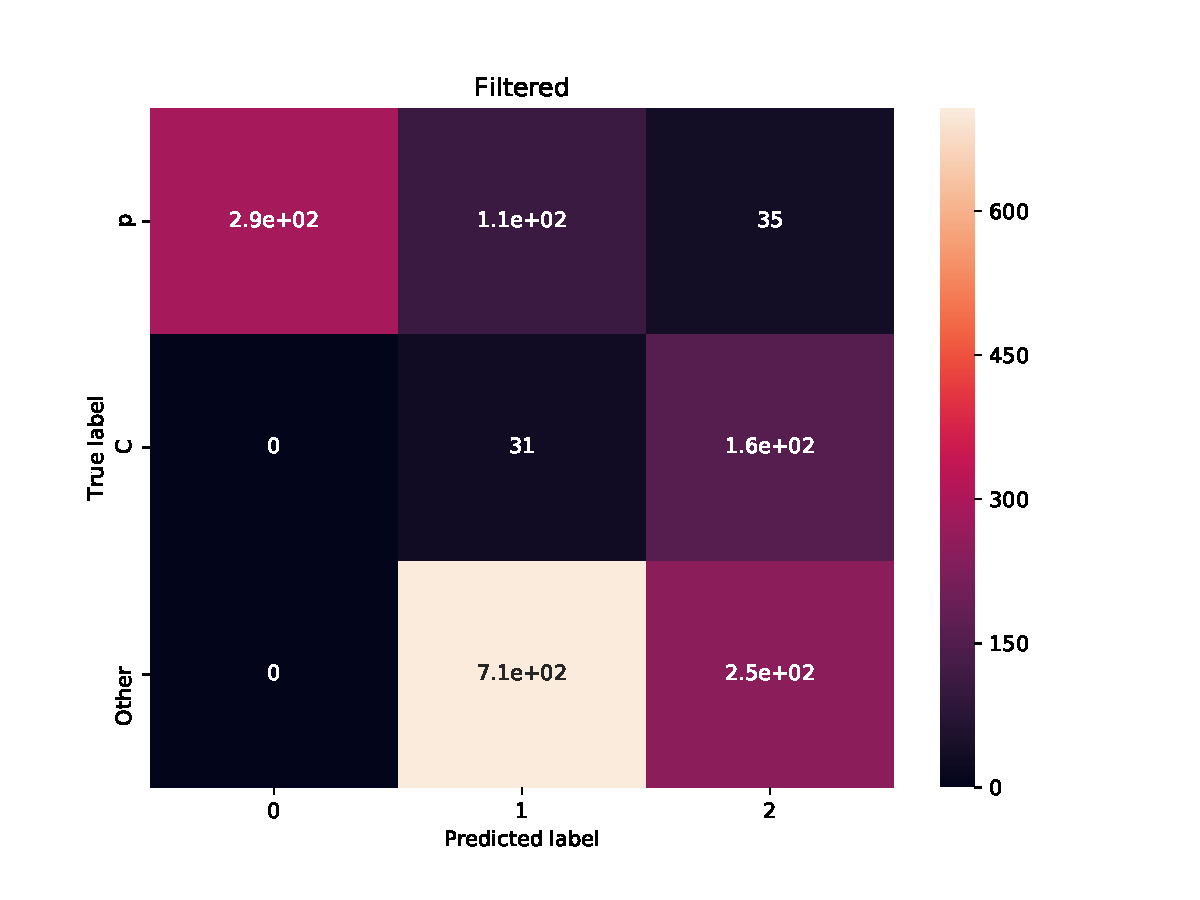
\includegraphics[width=0.35\textwidth]{plots/Filteredvgg_pca_conf_mat.pdf}
}
	\hspace{-1cm}
	\subfloat{
	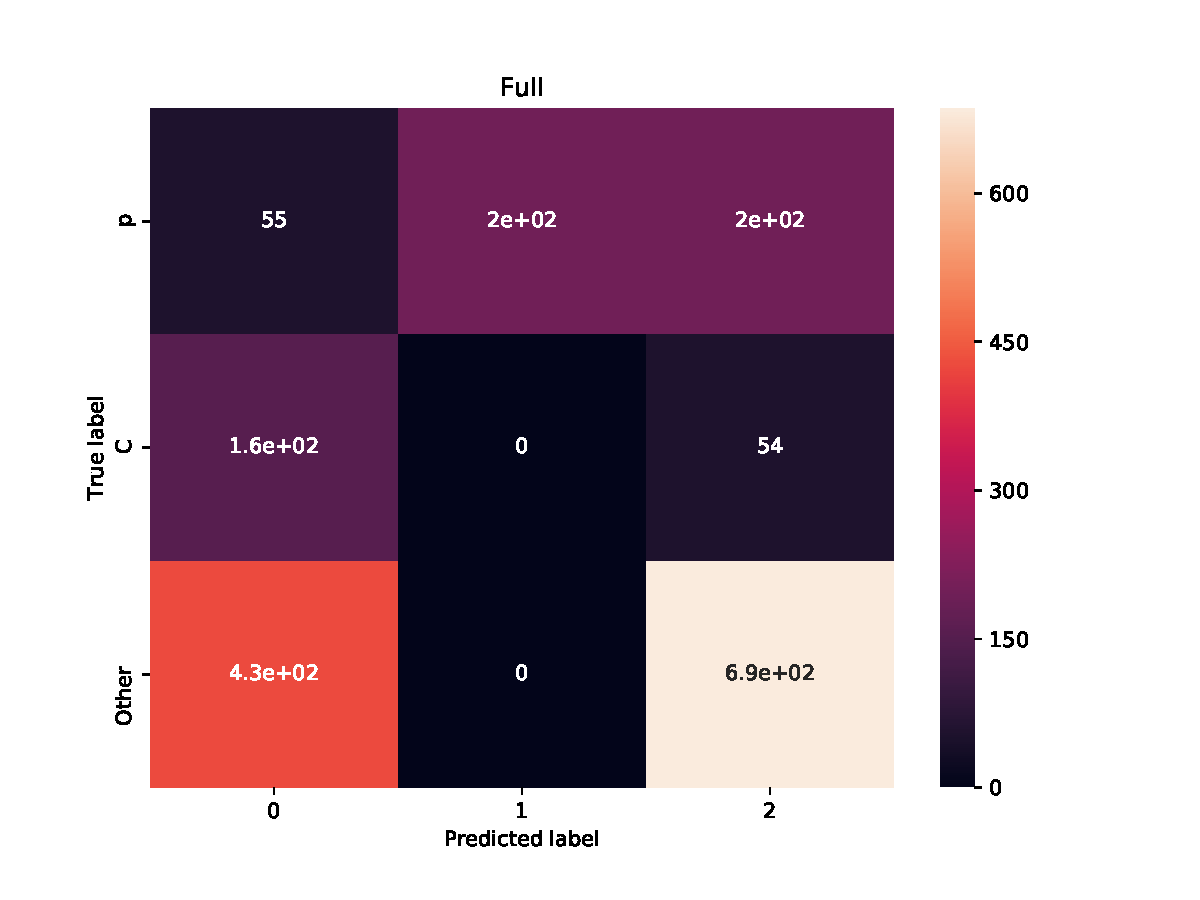
\includegraphics[width=0.35\textwidth]{plots/Fullvgg_pca_conf_mat.pdf}
}
\caption[Pre-trained network - confusion matrices]{Confusion matrices for the K-means clustering of simulated, filtered and full AT-TPC events. The true labels indicate samples belonging to the p (proton), carbon (C), or other classes. }\label{fig:clster_confmat}
\end{figure}

We repeat this analysis using a PCA dimensionality reduction on the latent space of the VGG16 model. This is done to estimate to what degree the class separating information is encoded in the entirety of the latent space, or in some select regions. The results from the PCA analysis were virtually identical to the results sans the PCA, and so we omit them for brevity. 

Furthermore, we wish to characterize further the clusters presented in figure \ref{fig:clster_confmat}. To achieve this, we sample from the proton samples belonging to different clusters for the filtered and full data.

\begin{figure}
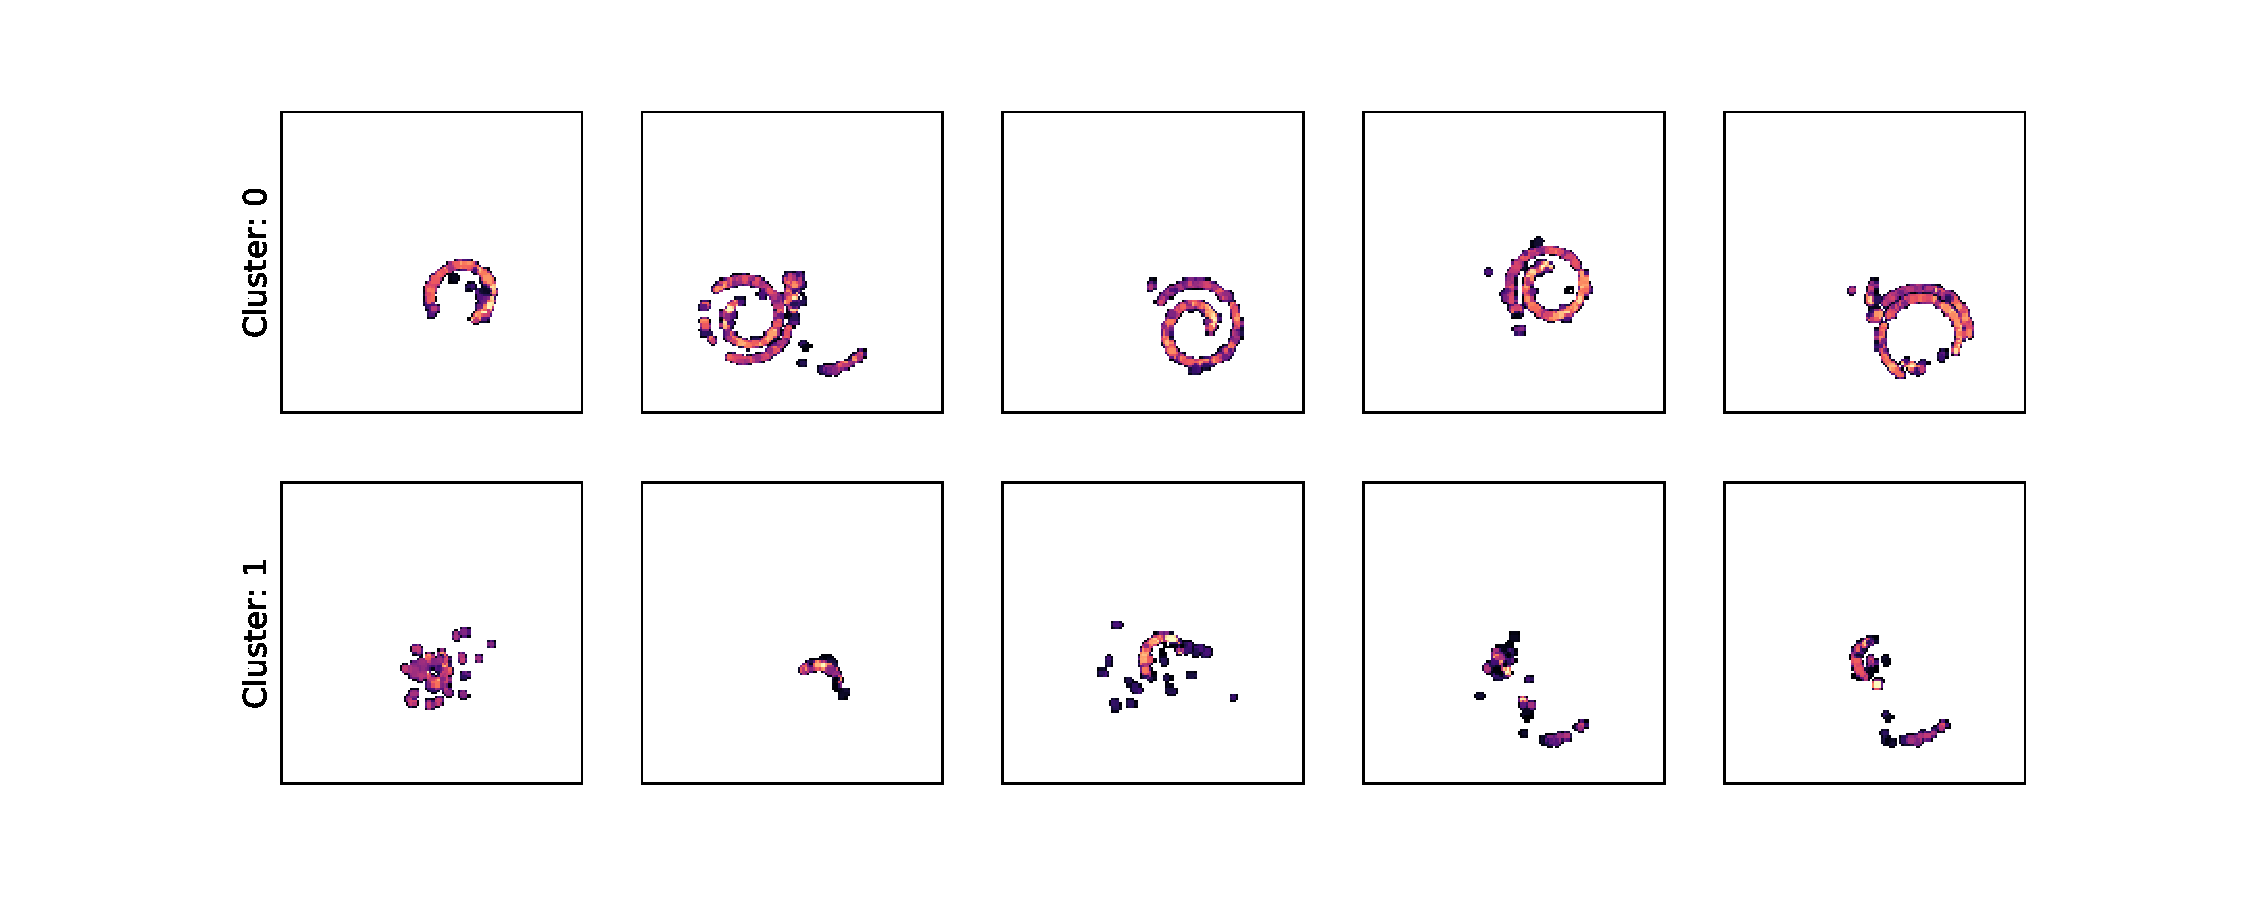
\includegraphics[width=\textwidth]{plots/filtered_vgg_cluster_repr.pdf}
\caption[Filtered proton samples by cluster belonging]{Illustrating a sample of proton events from different K-means clusters from the filtered dataset. Each row belongs to a single cluster corresponding to the filtered confusion matrix in figure \ref{fig:clster_confmat}}\label{fig:filtered_vgg_clster_repr}
\end{figure} 

\begin{figure}
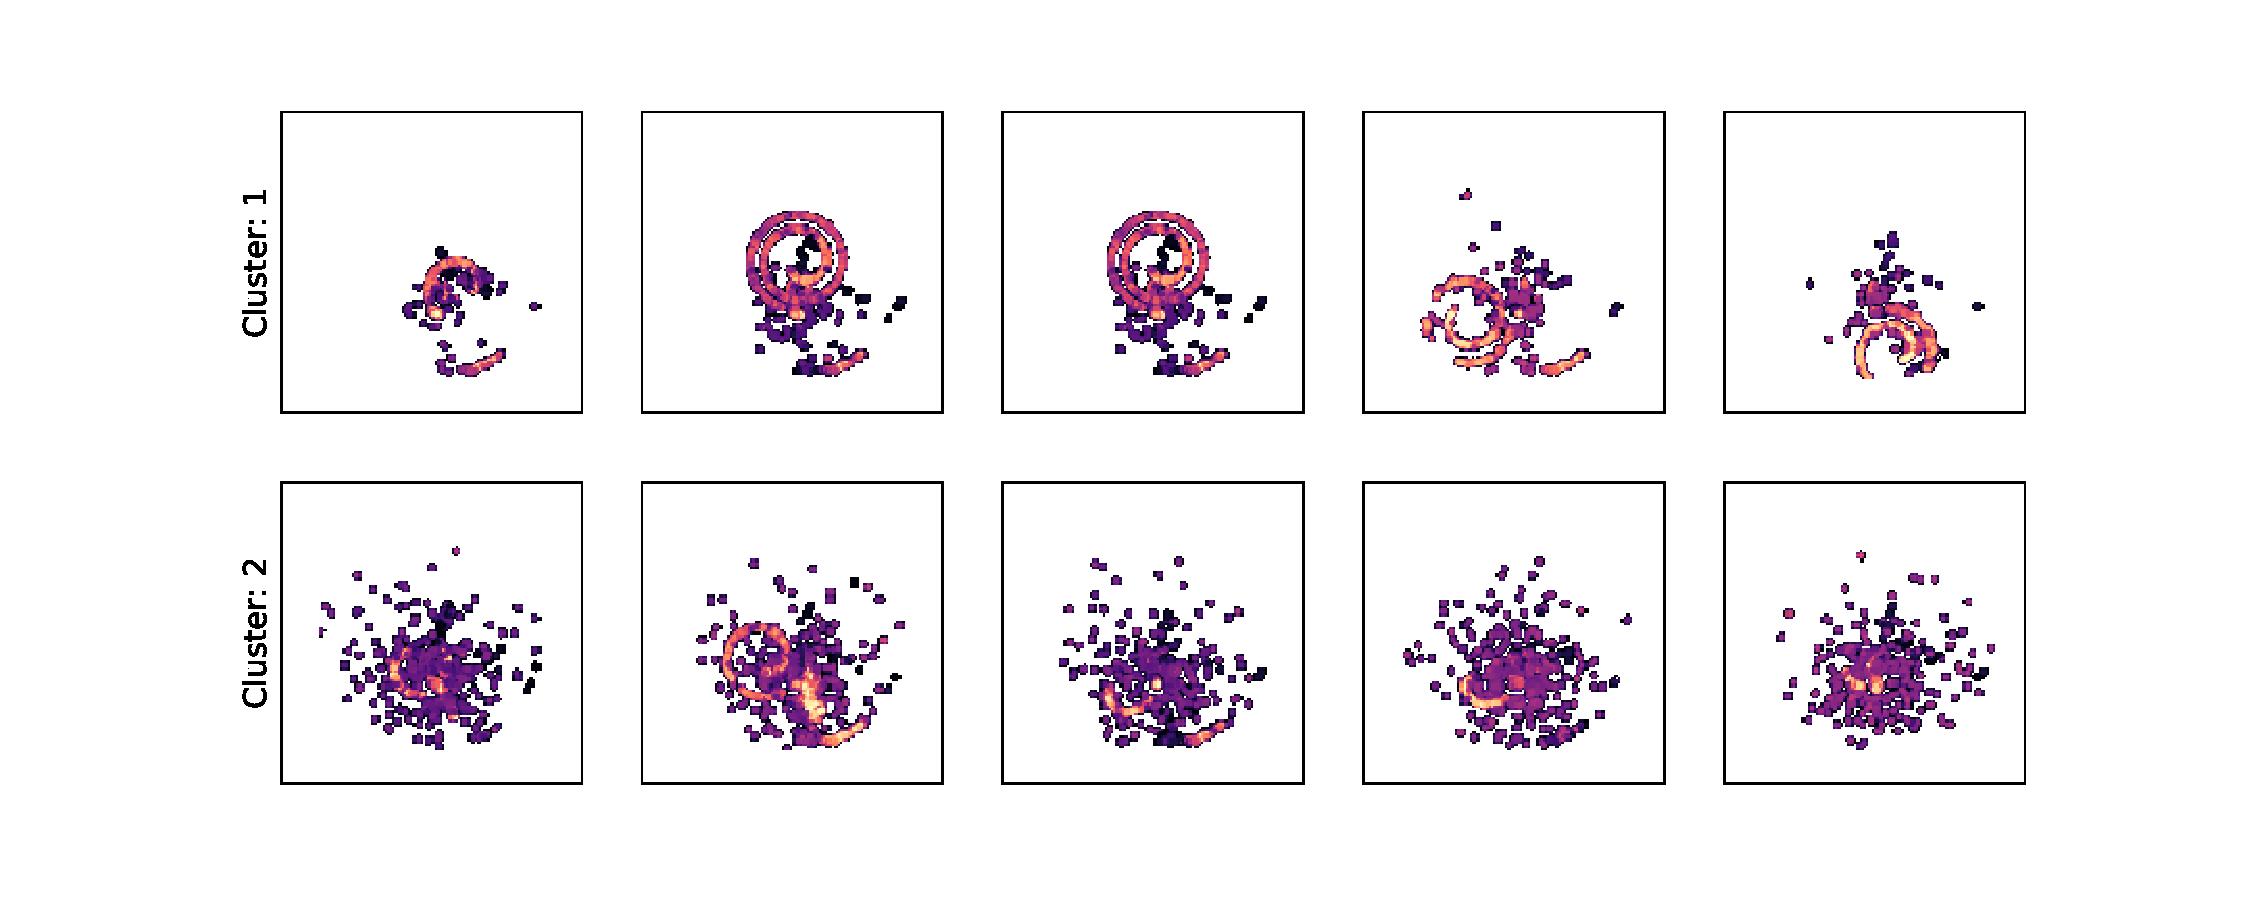
\includegraphics[width=\textwidth]{plots/full_vgg_cluster_repr.pdf}
\caption[Full proton samples by cluster belonging]{Illustrating a sample of proton events from different K-means clusters from the full dataset. Each row belongs to a single cluster corresponding to the full confusion matrix in figure \ref{fig:clster_confmat}}\label{fig:full_vgg_clster_repr}
\end{figure} 

In addition to the results presented in this section, we performed clustering with a number of different algorithms included in the \lstinline{scikit-learn} package. None of them provided any notable differences from the K-means results or were significantly worse. Notably, the DBSCAN algorithm failed to provide any useful clustering results. We find this important as one of the significant drawbacks of K-means, and the deep clustering algorithms presented in section \ref{sec:deep_clustering}, is that they are all dependent on pre-determining the number of clusters. This is not the case for DBSCAN. 
\subsection{Autoencoder clustering}

\section{Conclusions and Perspectives}\label{sec{conclusion}

\appendix  



\begin{thebibliography}{00}

%% \bibitem{label}
%% Text of bibliographic item

\bibitem{}

\end{thebibliography}
\end{document}
